\label{sec:eval}

We now evaluate   \oak's Java  implementation using synthetic benchmarks.
In \Cref{sec:druid} below, we discuss a real-world use case.

\subsection{Experiment setup} 

We generate a variety of workloads
using the popular synchrobench  tool~\cite{synchrobench}.
Our hardware testbed features an industry-standard 12-core Xeon E5-4650 CPU with 192 GB RAM. 

\paragraph{Compared solutions.} 
Our ultimate goal is to offer \oak\ as an alternative to Java's standard skiplist. 
We therefore compare it to the JDK8 ConcurrentSkipListMap~\cite{JavaSkipList},
which we refer to as \csl.  
%
To isolate the impact of off-heap allocation from other algorithmic aspects, 
we also implement  an off-heap variant of the Java skiplist, which we call \YoniList.
Note that whereas \csl\ offers an object-based API, \YoniList\ also exposes \oak's ZC API. 
Internally, \YoniList\/ 
maintains a concurrent skiplist over an intermediate {\em cell\/} object. Each cell references a key buffer 
and a value buffer allocated in off-heap arenas  through \oak's memory manager. 
%\YoniList\/ has a bigger on-heap footprint than \oak; however, its ZC API does not have the overhead of creating ephemeral objects upon reads. 
This solution is inspired by off-heap support  in production systems, e.g., HBase~\cite{HbaseOffheapWritePath}. 

{We also experimented with the open source concurrent off-heap B-tree implementation from MapDB~\cite{MapDB}, 
however it failed to scale to big datasets, peforming at least ten-fold slower than \oak; we omit these results for brevity.}

\paragraph{Methodology.}
The exercised keys and values are 100B- and 1KB-big, respectively. 
In each experiment, a specific \emph{range} of keys is accessed. 
Accessed keys are sampled  uniformly at random from that range. 
The range is used to control the dataset size:
Every experiment starts with an {\em ingestion\/} 
stage, which runs in a single thread and populates the KV-map with 50\% of the unique keys in the range 
using \algvar{putIfAbsent} operations. It is followed by the {\em sustained-rate\/} stage, 
which runs the target workload for 30 seconds through one or more symmetric worker threads. 
%
Every data point is the median of 3 runs; {the deviations among runs were all within 10\%}.
%All experiments exploit 32GB RAM, unless stated otherwise. 

In each experiment, all algorithms run with the same RAM budget. 
\oak\/ and \YoniList\/ split the available memory between the off-heap pool and the heap, 
allocating the former with just enough resources to host the raw data. \csl\/ allocates all the 
available memory to heap. 

% \paragraph{Configuration.}
We configure \oak\/ to use 4K entries per chunk, and invoke rebalance whenever the unsorted linked list
exceeds 0.5 of the sorted prefix. The  arena size is 100MB. 

\subsection{Results} 

\begin{figure*}[tb]
\centering
\begin{subfigure}[b]{0.33\linewidth}
\includegraphics[width=\textwidth]{figs/Ingestion.pdf}
\caption{Fixed RAM (32GB), varying dataset}
\label{fig:ingest:fixed_ram}
\end{subfigure}
\hspace{0.1\linewidth}
\begin{subfigure}[b]{0.33\linewidth}
\includegraphics[width=\textwidth]{figs/rev_Ingestion.pdf}
\caption{Fixed dataset (11GB), varying RAM}
\label{fig:ingest:fixed_data}
\end{subfigure}
\caption{Ingestion throughput scaling with RAM, single-threaded execution.}
\label{fig:memscale:ingestion}
\end{figure*}

\paragraph{Memory efficiency.}
We first study  how much of the available RAM can be utilized for the raw data, 
and how fast algorithms can perform within a given memory budget. 
Figure~\ref{fig:ingest:fixed_ram} depicts the  throughput of the ingestion stage 
with 32GB of RAM as the  number of ingested unique 
keys  goes up from 1M (approximately 1.1GB of raw data) to 20M (22GB). 
In Figure~\ref{fig:ingest:fixed_data}, we fix the dataset size to 10M KV-pairs (11GB), and vary the  
RAM budget from 15GB to 26GB.

First, we observe that the off-heap solutions can accommodate  bigger datasets within the same RAM,
and conversely, require less RAM to accommodate the same amount of data. 
For example, with 32GB of RAM,  \csl\/ caps at 15M KV-pairs while the off-heap solutions can accommodate 20M pairs.
This is due to the memory overhead for storing Java objects.
Note  that all algorithms deteriorate as the number of keys rises.
This happens because (1) the search time becomes  slower as the data structure grows, 
and (2) the Java GC overhead increases. 

Second, while the performance of on- and off-heap skiplists is  similar,  \oak\ is significantly faster, especially for large datasets.
There are multiple factors at play here. While off-heap solutions pay an overhead for 
copying all ingested data to off-heap buffers, they also eliminate much of the GC overhead. 
These effects cancel each other out. The  advantage of \oak\ then stems from its 
 locality-friendly data organization. % and low synchronization overhead.  


\paragraph{Scalability with parallelism.}
In the next set of experiments, we fix the available memory to 32GB and the ingested dataset size to 10M KV-pairs. 
We measure the sustained-rate stage throughput for multiple workloads, while scaling the number of worker threads from 1 to 12. 
In this setting, the raw data is less than 35\% of the available memory, i.e., %all algorithms enjoy a large on-heap headroom, hence 
the GC effect in all algorithms is minor. 

%We start from uniform workloads, each performing operations of a single type. 
Figure~\ref{fig:100_put} depicts the results of a put-only workload.
%(i.e., all operations are puts). 
\oak\/ scales 7.7x with 12 threads, while maintaining a 1.5x--1.9x throughput gap over \csl.  
\YoniList\/ is faster than \csl\/ but slower than \oak. 


Figure~\ref{fig:100_putifabsentcomputeifpresent} evaluates \oak's incremental update API, 
where each in-place update modifies 8 bytes of the value. 
In \csl, we invoke the (non-atomic) merge API.
\remove{
Since the Java API does not include \algvar{putIfAbsentComputeIfPresent}, we simulate it by calling first  \algvar{putIfAbsent},
and if it fails, locking the returned object and performing the computation. 
Since the lock is acquired only after 
\algvar{putIfAbsent} fails, the simulated operation is not atomic as in \oak.
}
In this experiment, 
\oak\/ scales 8x with 12 threads, and has 1.4x--1.6x higher throughput than \csl. 

Figure~\ref{fig:100_get} illustrates the get-only workload. Note that after calling get, an application can 
choose how much of the 1KB value to deserialize.  
To provide an upper bound on the impact of copying retrieved data, we also exercise the legacy API for \oak, which
copies the entire value.  We see that copying slows down \oak's performance by 30\%,
although, perhaps surprisingly, it is still faster than \csl. 
When refraining from copying, \oak\/ scales 10x with 12 threads, and consistently outperforms \csl\/ by 1.5x--1.6x.  
%The application-level gain may vary, depending on how much data the application deserializes 
%from the off-heap buffers. The legacy API, which copies all the data, provides the worst-case 
%performance. In this setting, the measured slowdown is approximately 30\% versus the ZC API, 
%which (surprisingly) is still faster than \csl. 
A mix of 95\% gets and 5\% puts (Figure~\ref{fig:put_get}) 
shows similar results: \oak\/ outperforms the competition by up to 1.75x.

\begin{figure*}[tb]
\centering
\begin{subfigure}[b]{0.33\linewidth}
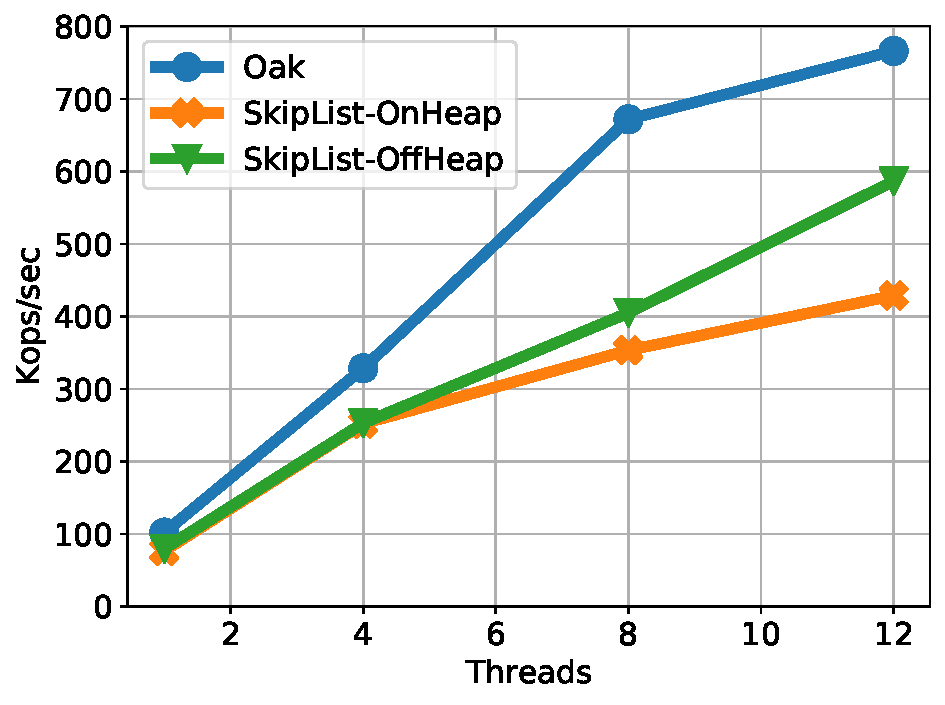
\includegraphics[width=\textwidth]{figs/micro_put-only.pdf}
\vskip -.1in
\caption{Put}
\label{fig:100_put}
\end{subfigure}
\begin{subfigure}[b]{0.33\linewidth}
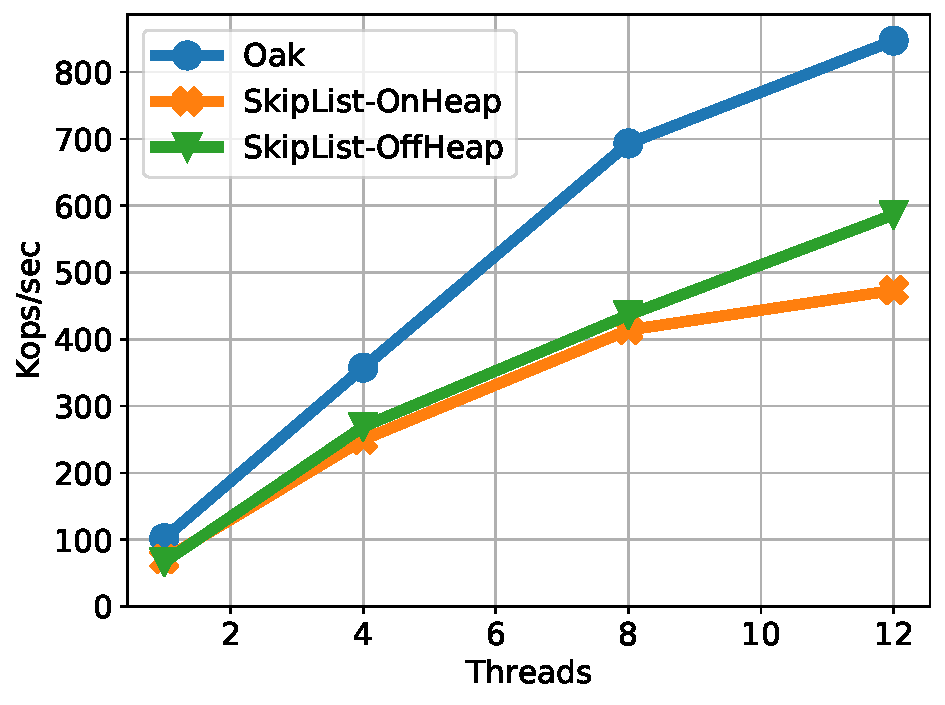
\includegraphics[width=\textwidth]{figs/micro_put-only-computeifpresent.pdf}
\vskip -.1in
\caption{PutIfAbsentComputeIfPresent}
\label{fig:100_putifabsentcomputeifpresent}
\end{subfigure}
\begin{subfigure}[b]{0.33\linewidth}
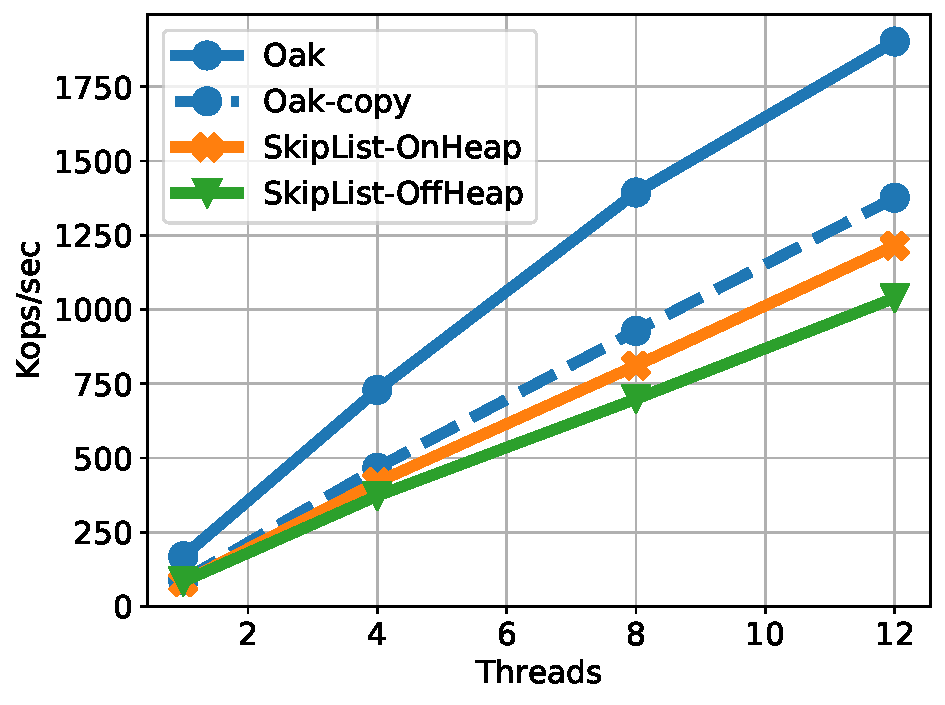
\includegraphics[width=\textwidth]{figs/micro_combined_get-only.pdf}
\vskip -.1in
\caption{Get}
\label{fig:100_get}
\end{subfigure}

\begin{subfigure}[b]{0.33\linewidth}
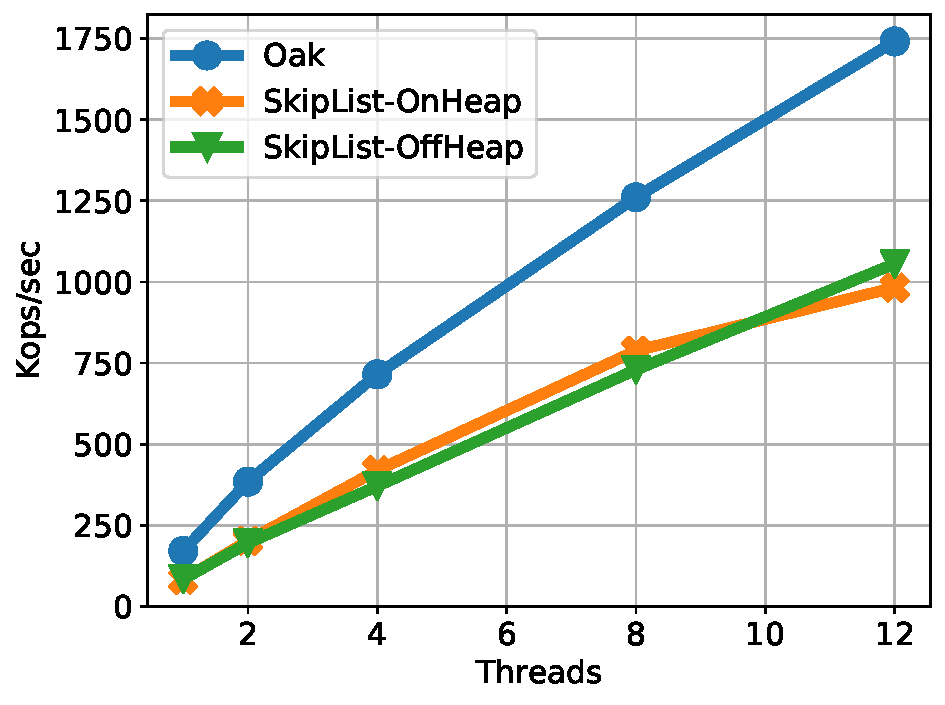
\includegraphics[width=\textwidth]{figs/put_get.pdf}
\vskip -.1in
\caption{95\% get, 5\% put} 
\label{fig:put_get}
\end{subfigure}
\begin{subfigure}[b]{0.33\linewidth}
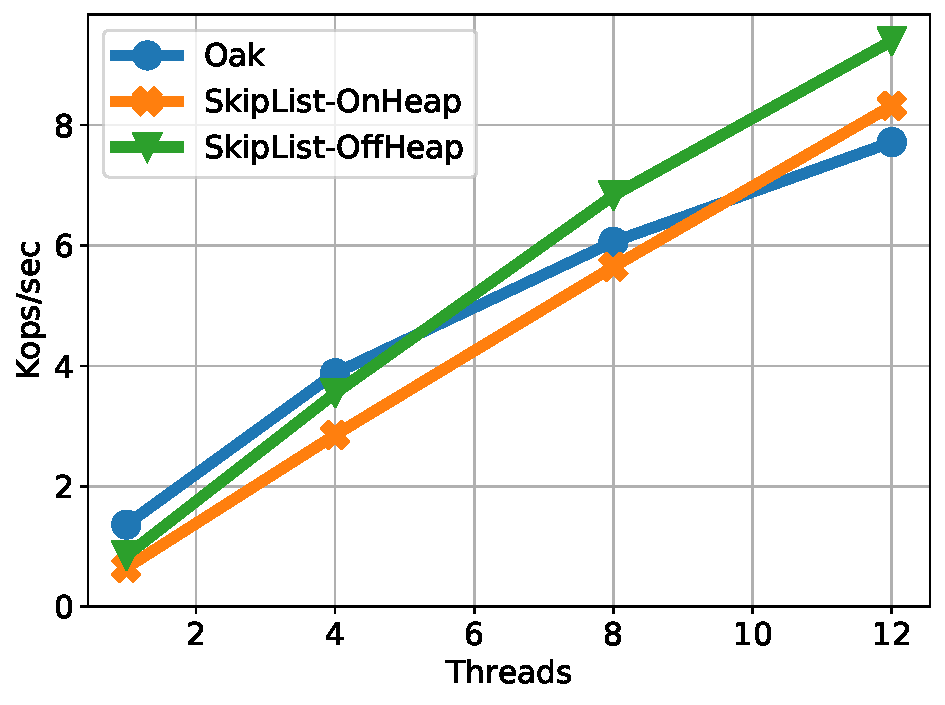
\includegraphics[width=\textwidth]{figs/micro_zc-ascend-only-10k.pdf}
\vskip -.1in
\caption{Scan (ascending), 10K values}
\label{fig:100_ascend_100}
\end{subfigure}
\begin{subfigure}[b]{0.33\linewidth}
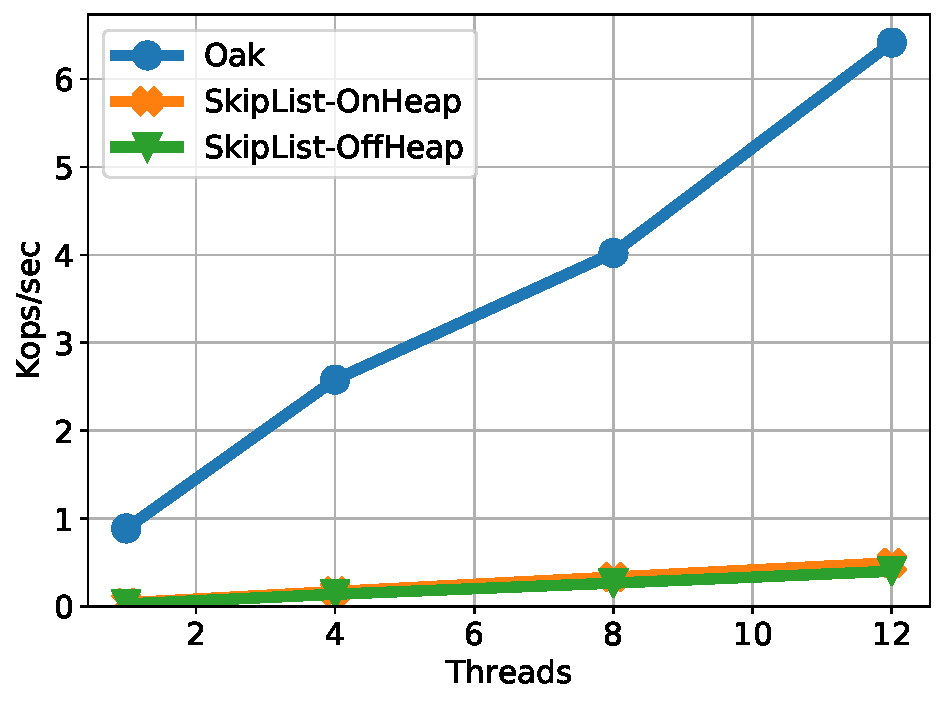
\includegraphics[width=\textwidth]{figs/micro_zc-descend-only-10k.pdf}
\vskip -.1in
\caption{Scan (descending), 10K values}
\label{fig:100_descend}
\end{subfigure}
\label{fig:throughput}
\caption{Sustained-rate throughput scaling with the the number of threads for uniform workloads, 11GB raw data.} 
\end{figure*}

We proceed to  ascending scans. 
%Figure~\ref{fig:100_ascend_10} focuses on short scans that traverse 10 key-value pairs.
Short scans, like gets, are dominated by the search time for the first KV-pair, and so we do not depict them separately. 
% -- e.g., \oak\/ traverses 10 values 40\% faster than \csl.  
Long scans, on the other hand, are dominated by the  iteration through the retrieved pairs.
In such scans, all three solutions perform similarly, as depicted in 
Figure~\ref{fig:100_ascend_100} for scans  traversing 10K values. 


\remove{
In this setting, \oak's performance is aggravated by creation of ephemeral OakRBuffer objects for 
each traversed entity (key, value, or both, depending on the API), whereas its competitors 
only retrieve references to existing objects. Figure~\ref{fig:100_ascend_100} depicts the behavior 
of scans that retrieve either 100 values (solid curve) of 100 KV-pairs (dashed curve). For the former, 
\oak\/ is approximately 20\% faster than \csl\/ (and also \YoniList), whereas for the latter it is 20\% slower, 
as it creates twice as many objects. If the application performs some computation in addition to the raw 
scan, these gaps become immaterial.}

%the overhead of ephemeral object creation and the associated GC are noticeable
%The above results are for raw scan throughput, which does not take any steps during the iteration. 
%We next investigate a scenario where the application executes some computation steps 
%after each key-value pair it retrieves. We use a scan to summarize 100 values, accessing 8 bytes in each of them. 
%As Figure~\ref{fig:100_ascend_compute_100} shows, {\inred {TBC -- wait for Yoni's results.}}
%We studied even longer scans (up to 10K entries), and observed similar throughput losses. %of up to 30\%. 
%Note that Oak has not been designed for this high-intensity read-only setting. %application developers could use a different data structure in this case. 

Finally, Figure~\ref{fig:100_descend} depicts the performance of descending scans over 10K values. 
We see that \oak's efficient chunk-based descending scans are almost as fast as its ascending scans. 
\oak\ exhibits a huge advantage over the competition, outperforming both skiplists more than tenfold. 





 